\documentclass[10pt, a4paper]{beamer}

\usetheme{Berkeley}
\usecolortheme{sidebartab}

\begin{document}
	\setbeamertemplate{sidebar left}{}
	\title{Progress Presentation-I}
	\subtitle{e-Yantra Summer Intership-2017 \\Comparison Study of Traditional Way of Programming
		Firebird with the Statechart Based Model of
		Programming}
	\author{Manav Guglani\\
	Mentor: Naveen C}
	\institute{IIT Bombay}
	\date{\today}
	%\addtobeamertemplate{sidebar left}{}{\includegraphics[scale = 0.3]{logowithtext.png}}
	\frame{\titlepage}

\setbeamertemplate{sidebar left}[sidebar theme]
\section{Overview of Project}
\begin{frame}{Overview of Project}
	\begin{itemize}
		\item Project Name:- Comparison Study of Traditional Way of Programming
		Firebird with the Statechart Based Model of
		Programming
		\item Objective
		\begin{enumerate}
			\item Modelling of robotic themes using statecharts
			\item Platform independent code generation
			\item Comparison study
		\end{enumerate}
		\item Deliverables
		\begin{enumerate}
			\item Statechart models for various tasks
			\item Report containing comparison study
		\end{enumerate}
	\end{itemize}
\end{frame}

\section{Overview of Task}
\begin{frame}{Overview of Task}
\begin{table}[]
	\centering
	\caption{My caption}
	\label{my-label}
	\resizebox{\textwidth}{!}{%
		\begin{tabular}{|l|l|l|}
			\hline
			Task no. & Task & Deadline \\ \hline
			1 & Learn Syntax and Semantics of Statecharts asdescribed by David Harel. & 3 days \\ \hline
			2 & Understanding the existing standard statechart models of some systems. & 3 days \\ \hline
			3 & \begin{tabular}[c]{@{}l@{}}Model some of the tasks given to students in e-yantra competition \\ using statecharts.\end{tabular} & 10 days \\ \hline
			4 & Explore the statechart Editor tool Yakindu. & 2 days \\ \hline
			5 & Model the tasks using Yakindu and integrate with firebird libraries & 4 days \\ \hline
			6 & Writing the same code manually for the respective robotic tasks & 12-14 days \\ \hline
			7 & \begin{tabular}[c]{@{}l@{}}Compare the cycle time for Manually written code and \\ Yakindu generated code.\end{tabular} & 1 day \\ \hline
			8 & \begin{tabular}[c]{@{}l@{}}Comment on how to make the yakindu generated code \\ efficient and how to make the software components reusable\end{tabular} & 3 days \\ \hline
			9 & Report and presentation & 4 days \\ \hline
		\end{tabular}%
	}
\end{table}
\end{frame}

\section{Task Accomplised}
\begin{frame}{Task Accomplised}
	\begin{itemize}
		\item Learned Syntax and Semantics of Statecharts as
		described in David Harel's paper
		\begin{enumerate}
			\item Clustering
			\item Orthogonality
			\item Broadcast Communication
		\end{enumerate}
		\item understood some of the existing statechart models
		\begin{enumerate}
			\item Line follower robot
			\item Obstacle avoider robot
			\item Citizen
			Quartz Multi-Alarm III wristwatch
			\item Valet Parking
		\end{enumerate}
	\item Explored statechart editor tool Yakindu. (made some models in it).
	\end{itemize}

\end{frame}
\begin{frame}{sequence detector - 1011}
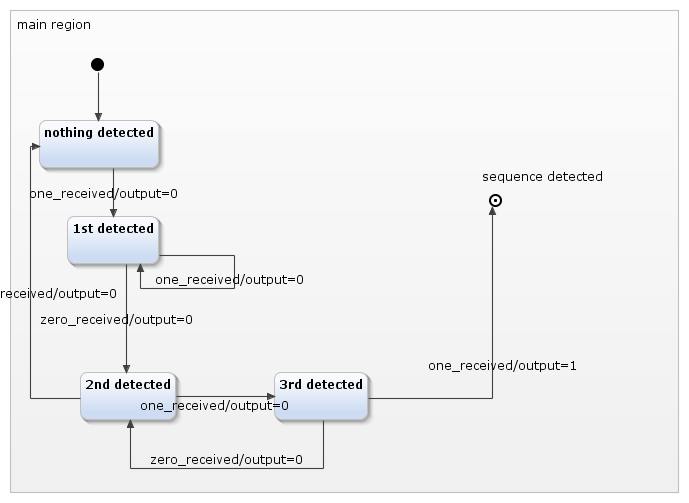
\includegraphics[width=11cm, height=8.38cm]{sequence1011.png}
\end{frame}

\begin{frame}{obstacle avoider}
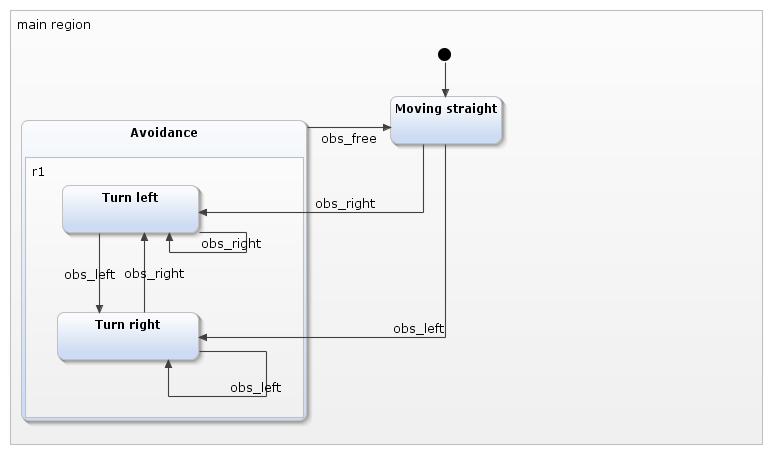
\includegraphics[width=11.04cm, height=6.5cm]{obstacle_avoider.png}
\\
Reference:- http://web.stanford.edu/class/cs123/lectures/
\end{frame}

\begin{frame}{Multiple Timers}
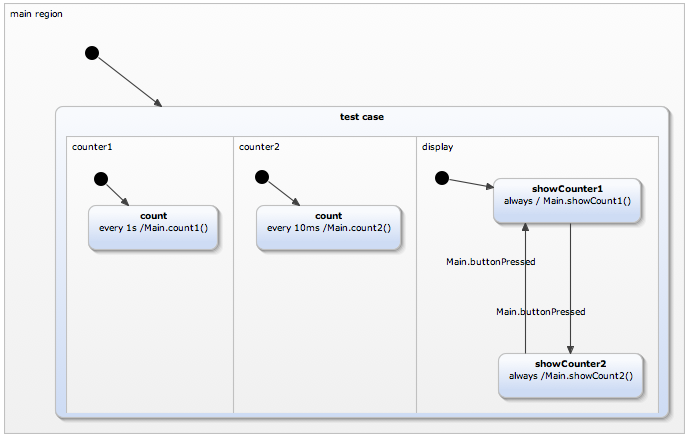
\includegraphics[width=11.48cm, height=7.3cm]{ortho.png}
\\
Reference:- google groups
\end{frame}

\section{Challenges Faced}
\begin{frame}{Challenges Faced}
	\begin{itemize}
		\item Understanding the statechart model of the watch given in David Harel's paper. (Contains lots of clustered states and orthogonal states with a lot of nesting and dependencies). 
	\end{itemize}
\end{frame}

\section{Future Plans}
\begin{frame}{Future Plans for presentation 2}
	\begin{itemize}
		\item Modelling some of the tasks given to students in e-yantra
		competition using statecharts.
		\item Modelling the tasks using Yakindu and integrate with
		firebird libraries
		\item Comparison study
	\end{itemize}
\end{frame}


\section{Thank You}
\begin{frame}{Thank You}
	\centering THANK YOU !!!
\end{frame}
\end{document}
